\chapter{Introduzione ai DBMS}

\section*{Introduzione}
Un Database Management System (DBMS) è un software specializzato che gestisce la memorizzazione, l'organizzazione e l'accesso ai dati. Questo capitolo introduce i concetti fondamentali dei sistemi informativi e le proprietà ACID che garantiscono l'affidabilità dei dati.

\section*{Obiettivi di apprendimento}
\begin{itemize}
    \item Comprendere la differenza tra dati e informazioni
    \item Conoscere i componenti di un sistema informativo
    \item Capire il ruolo di un DBMS
    \item Apprendere le proprietà ACID delle transazioni
    \item Identificare vantaggi e caratteristiche dei DBMS
\end{itemize}

\section{Dati, Informazioni e Sistemi Informativi}

\subsection{Differenza tra dati e informazioni}
I \textbf{dati} sono fatti grezzi e non strutturati. Le \textbf{informazioni} sono dati elaborati e organizzati che hanno significato e utilità.

\begin{tcolorbox}[colback=blue!10, colframe=blue!60, title=Esempio: Dati vs Informazioni]
\textbf{Dato}: \texttt{25, 1990, Milano, Rossi}

\textbf{Informazione}: Il cliente Luigi Rossi, nato nel 1990 a Milano, ha 25 anni ed è residente in Lombardia.
\end{tcolorbox}

\subsection{Componenti di un sistema informativo}
Un sistema informativo è composto da diversi elementi interdipendenti che lavorano insieme. L'infrastruttura hardware fornisce la base fisica con computer, server e dispositivi di storage. Il software, che include applicazioni, DBMS e sistemi operativi, gestisce l'elaborazione e l'accesso ai dati. I dati stessi rappresentano il patrimonio informativo dell'organizzazione, fondamentale per le decisioni aziendali. I processi definiscono le operazioni e le procedure aziendali che trasformano i dati in informazioni utili. Infine, le risorse umane—amministratori, sviluppatori e utenti—sono essenziali per progettare, mantenere e utilizzare il sistema informativo in modo efficace.

\section{Database Management System (DBMS)}

\subsection{Definizione e ruolo}
Un DBMS è un software specializzato che offre una serie di funzionalità critiche per la gestione dei dati. Consente di memorizzare dati in modo organizzato e persistente, assicurando che le informazioni rimangono disponibili nel tempo. Facilita il recupero efficiente dei dati tramite query ottimizzate e indici. Permette di aggiornare i dati mantenendo la coerenza e l'integrità secondo regole definite. Un DBMS fornisce anche un sofisticato controllo degli accessi, limitando chi può leggere o modificare determinati dati. Infine, protegge i dati da accessi non autorizzati attraverso meccanismi di autenticazione e crittografia.

\subsection{Vantaggi del DBMS}
\begin{tcolorbox}[colback=green!10, colframe=green!60, title=Vantaggi chiave]
\begin{itemize}
    \item \textbf{Centralizzazione}: un'unica fonte di verità
    \item \textbf{Efficienzaad accesso}: strutture dati ottimizzate
    \item \textbf{Sicurezza}: controllo degli accessi e crittografia
    \item \textbf{Affidabilità}: backup e recovery automatici
    \item \textbf{Integrità}: regole e vincoli garantiscono coerenza
    \item \textbf{Scalabilità}: gestisce grandi volumi di dati
    \item \textbf{Concorrenza}: accesso multiplo simultaneo
\end{itemize}
\end{tcolorbox}

\section{Le proprietà ACID}

\subsection{Proprietà ACID delle transazioni}
Una transazione è una sequenza di operazioni che costituisce un'unità di lavoro logica. Le proprietà ACID garantiscono l'affidabilità:

\begin{description}
    \item[\textbf{A - Atomicità}] La transazione è indivisibile: si esegue completamente o non si esegue per nulla (all-or-nothing).
    \item[\textbf{C - Coerenza}] Lo stato del database deve rimanere coerente prima e dopo la transazione.
    \item[\textbf{I - Isolamento}] Transazioni concorrenti non si interferiscono l'una con l'altra.
    \item[\textbf{D - Durabilità}] Una volta eseguita, una transazione persiste anche in caso di guasto.
\end{description}

\subsection{Atomicità}
Ogni transazione è atomica: non può rimanere nello stato intermedio.

\begin{tcolorbox}[colback=red!10, colframe=red!60, title=Attenzione: Problema senza atomicità]
Trasferimento di 100 euro tra due conti. Se il sistema crasha dopo il prelievo ma prima del deposito, il denaro è perso!
\end{tcolorbox}

\subsection{Coerenza}
Il database mantiene regole e vincoli di integrità.

\begin{lstlisting}[language=SQL, caption=Esempio: Vincolo di coerenza]
-- Il saldo non può mai essere negativo
ALTER TABLE conto ADD CONSTRAINT saldo_positivo
    CHECK (saldo >= 0);
\end{lstlisting}

\subsection{Isolamento}
Transazioni concorrenti non si vedono i reciproci effetti intermedi.

\begin{tcolorbox}[colback=orange!10, colframe=orange!60, title=Nota: Livelli di isolamento]
Existono diversi livelli di isolamento (READ UNCOMMITTED, READ COMMITTED, REPEATABLE READ, SERIALIZABLE) per bilanciare performance e sicurezza.
\end{tcolorbox}

\subsection{Durabilità}
I dati sono permanentemente memorizzati.

\begin{lstlisting}[language=SQL, caption=Esempio: Commit garantisce durabilità]
START TRANSACTION;
UPDATE conto SET saldo = saldo - 100 WHERE id = 1;
UPDATE conto SET saldo = saldo + 100 WHERE id = 2;
COMMIT; -- I dati sono ora permanenti
\end{lstlisting}

\section{Tipi di DBMS}

\subsection{DBMS Relazionali}
Organizzano i dati in tabelle con relazioni tra loro. Esempi: MySQL, PostgreSQL, Oracle, SQL Server.

\subsection{DBMS NoSQL}
Memorizzano dati in formato non relazionale. Esempi: MongoDB, Cassandra, Redis.

\subsection{DBMS NewSQL}
Combinano vantaggi relazionali e NoSQL. Esempi: CockroachDB, TiDB.

\section{Architettura di un DBMS}

\begin{figure}[h]
    \centering
    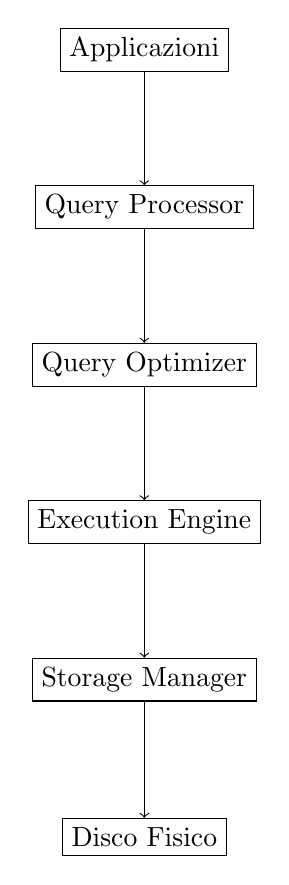
\begin{tikzpicture}[node distance=2cm]
        \node[draw, rectangle] (app) {Applicazioni};
        \node[draw, rectangle, below of=app] (query) {Query Processor};
        \node[draw, rectangle, below of=query] (optim) {Query Optimizer};
        \node[draw, rectangle, below of=optim] (exec) {Execution Engine};
        \node[draw, rectangle, below of=exec] (storage) {Storage Manager};
        \node[draw, rectangle, below of=storage] (disk) {Disco Fisico};

        \draw[->] (app) -- (query);
        \draw[->] (query) -- (optim);
        \draw[->] (optim) -- (exec);
        \draw[->] (exec) -- (storage);
        \draw[->] (storage) -- (disk);
    \end{tikzpicture}
    \caption{Architettura a livelli di un DBMS}
\end{figure}

\section*{Riepilogo concetti chiave}

\begin{tcolorbox}[colback=gray!10, colframe=black!60, title=Concetti fondamentali]
Un \textbf{DBMS} è lo strumento essenziale per centralizzare e gestire i dati di un'organizzazione in modo professionale. Le proprietà \textbf{ACID} sono il fondamento che garantisce transazioni affidabili e coerenti. L'\textbf{atomicità} assicura il principio del tutto-o-nulla, dove una transazione si completa interamente o non avviene affatto. La \textbf{coerenza} mantiene l'integrità dei vincoli durante tutte le operazioni. L'\textbf{isolamento} separa le transazioni concorrenti impedendo interferenze reciproche. Infine, la \textbf{durabilità} rende i dati permanenti e protetti anche di fronte a guasti imprevisti di sistema.
\end{tcolorbox}

\section*{Esercizi}

\begin{enumerate}
    \item Spiega con un esempio concreto la differenza tra data e informazione.

    \item Descrivi come le proprietà ACID garantiscono un trasferimento bancario sicuro tra due conti.

    \item Un'operazione di trasferimento fallisce a metà. Quale proprietà ACID evita che il denaro scompaia? Spiega.

    \item Elenca almeno tre vantaggi di un DBMS rispetto a un archivio basato su file di testo.

    \item Qual è la differenza tra DBMS relazionali e NoSQL? Fai un esempio di situazione dove sceglieresti l'uno o l'altro.
\end{enumerate}
